% begin module polar-to-cartesian
\begin{frame}
\begin{itemize}
\item  How do we go from polar coordinates to Cartesian coordinates?
\item<2->  Suppose a point has polar coordinates $(r, \theta )$ and Cartesian coordinates $(x,y)$.
\item<8->  How do we go from Cartesian coordinates to polar coordinates?
\end{itemize}
\begin{columns}[c]
\column{.6\textwidth}
\ \uncover<2->{%
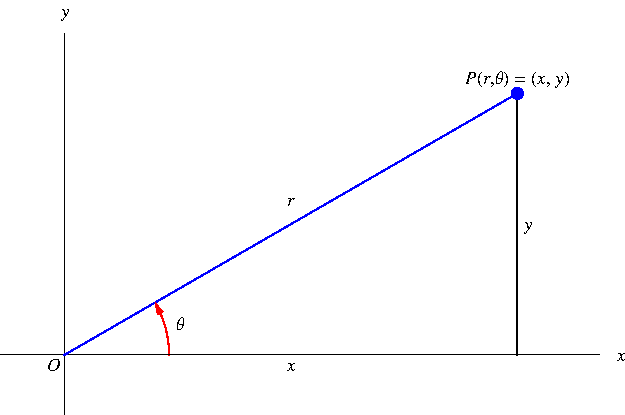
\includegraphics[height=5cm]{polar-curves/pictures/11-03-conversion.pdf}%
}%
\column{.4\textwidth}
\[
\uncover<3->{%
\alert<handout:0| 3-4>{\cos\theta = \uncover<4->{\frac{x}{r}}}\qquad %
}%
\uncover<3->{%
\alert<handout:0| 5-6>{\sin\theta = \uncover<6->{\frac{y}{r}}}%
}%
\]
\[
\uncover<7->{%
x = r\cos \theta \qquad y = r\sin \theta
}%
\]
\[
\uncover<9->{%
\alert<handout:0| 9-10>{r^2 = \uncover<10->{x^2 + y^2}}\qquad %
}%
\]
\end{columns}
\end{frame}
% end module polar-to-cartesian
